% Auto-generated by paper/figures/generate.py
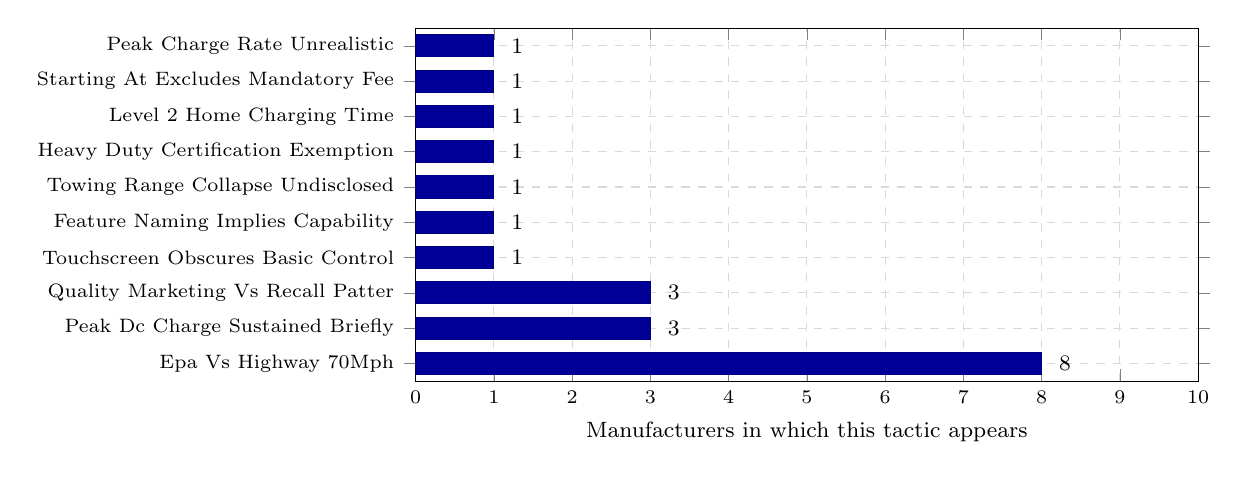
\begin{tikzpicture}
  \begin{axis}[
      width=0.95\textwidth, height=0.5\textwidth,
      xbar, xmin=0, xmax=10,
      ymin=0.5, ymax=10.5,
      ytick={1,2,3,4,5,6,7,8,9,10}, yticklabels={Epa Vs Highway 70Mph,Peak Dc Charge Sustained Briefly,Quality Marketing Vs Recall Patter,Touchscreen Obscures Basic Control,Feature Naming Implies Capability,Towing Range Collapse Undisclosed,Heavy Duty Certification Exemption,Level 2 Home Charging Time,Starting At Excludes Mandatory Fee,Peak Charge Rate Unrealistic},
      xlabel={Manufacturers in which this tactic appears},
      tick label style={font=\scriptsize},
      xlabel style={font=\footnotesize},
      bar width=8pt,
      grid=major, grid style={dashed,gray!30},
    ]
    \addplot[fill=blue!60!black, draw=blue!50!black] coordinates {(8,1) (3,2) (3,3) (1,4) (1,5) (1,6) (1,7) (1,8) (1,9) (1,10)};
    \node[anchor=west, font=\footnotesize] at (axis cs:8.1,1) {8};
    \node[anchor=west, font=\footnotesize] at (axis cs:3.1,2) {3};
    \node[anchor=west, font=\footnotesize] at (axis cs:3.1,3) {3};
    \node[anchor=west, font=\footnotesize] at (axis cs:1.1,4) {1};
    \node[anchor=west, font=\footnotesize] at (axis cs:1.1,5) {1};
    \node[anchor=west, font=\footnotesize] at (axis cs:1.1,6) {1};
    \node[anchor=west, font=\footnotesize] at (axis cs:1.1,7) {1};
    \node[anchor=west, font=\footnotesize] at (axis cs:1.1,8) {1};
    \node[anchor=west, font=\footnotesize] at (axis cs:1.1,9) {1};
    \node[anchor=west, font=\footnotesize] at (axis cs:1.1,10) {1};
  \end{axis}
\end{tikzpicture}
